\documentclass[12pt]{article}

\usepackage{sbc-template}
\usepackage{graphicx,url}
\usepackage[utf8]{inputenc}
\usepackage[brazil]{babel}

\sloppy

\title{Classificação de alimentos com EfficientNet-B0}

\author{Eduardo de Medeiros da Silveira\inst{1}}

\address{Centro de Tecnologia -- Universidade Federal de Santa Maria (UFSM)\\
  Av. Roraima, nº 1000 -- Cidade Universitária -- Bairro Camobi\\
  97105-900 -- Santa Maria -- RS -- Brasil
  \email{eduardomsilveira3@gmail.com}
}

\begin{document}

\maketitle

\begin{abstract}
  This study investigates food classification on Food-101 using an
  ImageNet-pretrained EfficientNet-B0. Four configurations are compared:
  classifier training, Batch Normalization statistics adaptation, additional
  training of its scale and shift parameters, and Stochastic Depth activation.
  Convolutional weights remain frozen in all experiments. The evaluation uses
  the same training, validation, and test splits, top-1 and top-5 accuracy,
  and per-class error analysis
  to assess these strategies. Training Batch Normalization parameters with
  Stochastic Depth achieved the best test accuracy: 79.43\% top-1 and
  94.86\% top-5.
\end{abstract}

\begin{resumo}
  Este trabalho investiga a classificação de alimentos no Food-101 com uma
  EfficientNet-B0 pré-treinada no ImageNet. Comparam-se quatro configurações:
  treinamento do classificador, adaptação das estatísticas do Batch
  Normalization, treinamento adicional de seus parâmetros de escala e
  deslocamento e ativação do Stochastic Depth. Os pesos das convoluções
  permanecem congelados. A avaliação utiliza a mesma divisão dos dados em
  treino, validação e teste,
  acurácias top-1 e top-5 e análise dos erros por classe para investigar os
  efeitos dessas estratégias. O treinamento dos parâmetros do Batch
  Normalization com Stochastic Depth obteve as maiores acurácias de teste:
  79,43\% top-1 e 94,86\% top-5.
\end{resumo}

\section{Introdução}
\label{sec:introducao}

A classificação automática de alimentos consiste em identificar a categoria
de um alimento a partir de sua imagem. Essa tarefa apresenta desafios devido
à variação de aparência dentro de uma mesma classe e à semelhança visual entre
classes distintas. Diferentes formas de preparo, apresentação, iluminação e
enquadramento podem dificultar o reconhecimento. Neste trabalho, o problema
é tratado como uma tarefa de classificação supervisionada multiclasse, na qual
cada imagem deve ser associada a uma das 101 categorias do conjunto
Food-101~\cite{bossard2014food101}.

A abordagem adotada utiliza transferência de aprendizado com uma
EfficientNet-B0~\cite{tan2019efficientnet} pré-treinada no ImageNet. Sua camada
de classificação é substituída para atender às categorias do Food-101,
preservando os pesos das convoluções. Essa configuração permite investigar
a adaptação de uma rede pré-treinada ao reconhecimento de alimentos sem
ajustar todos os seus parâmetros.

O objetivo do estudo é avaliar o efeito de diferentes configurações de
Batch Normalization e Stochastic Depth sobre o desempenho de classificação.
São comparados quatro experimentos: treinamento apenas do classificador;
atualização adicional das médias e variâncias do Batch Normalization;
treinamento também de seus parâmetros de escala e deslocamento; e ativação
do Stochastic Depth nessa última configuração. A comparação utiliza a mesma
divisão de dados e considera as acurácias top-1 e top-5, além da análise dos
erros por classe.

\section{Dataset e preparação dos dados}
\label{sec:dataset}

O Food-101 reúne 101.000 imagens de alimentos, distribuídas igualmente entre
101 classes. A divisão oficial contém 750 imagens de treinamento e 250 de
teste por classe. As imagens de teste foram revisadas manualmente, enquanto
o conjunto de treinamento preserva ruídos, incluindo exemplos com rótulos
incorretos~\cite{bossard2014food101}. Neste trabalho, os dados são carregados
pela biblioteca Hugging Face Datasets, a partir do repositório
\texttt{ethz/food101}\footnote{\url{https://huggingface.co/datasets/ethz/food101}}.

O repositório disponibiliza dois subconjuntos, denominados \texttt{train} e
\texttt{validation}. O subconjunto original \texttt{train}, com 75.750
imagens, foi dividido em dois novos conjuntos: 80\% para treino e 20\% para
validação, com estratificação por classe e semente aleatória 42. Já o
subconjunto original \texttt{validation}, com 25.250 imagens, foi utilizado
integralmente como conjunto de teste, reservado para a avaliação final.
Portanto, a
validação utilizada durante o treinamento foi extraída exclusivamente do
\texttt{train} original. A
Tabela~\ref{tab:divisao-dados} apresenta a divisão utilizada nos quatro
experimentos. Os subconjuntos são disjuntos, e a validação é avaliada ao final
de cada época. Como a validação deriva do conjunto original de treinamento,
ela também pode conter rótulos incorretos.

\begin{table}[ht]
  \centering
  \caption{Distribuição das imagens nos subconjuntos do experimento.}
  \label{tab:divisao-dados}
  \begin{tabular}{lrr}
    \hline
    Subconjunto & Total de imagens & Imagens por classe \\
    \hline
    Treino & 60.600 & 600 \\
    Validação & 15.150 & 150 \\
    Teste & 25.250 & 250 \\
    \hline
  \end{tabular}
\end{table}

O pré-processamento é o mesmo nos três subconjuntos. As imagens são
redimensionadas para que o menor lado tenha 256 pixels, preservando a
proporção original e utilizando interpolação bicúbica. Em seguida, aplica-se
um recorte central de $224 \times 224$ pixels. Os valores dos pixels são
convertidos para ponto flutuante de 32 bits e escalados para $[0,1]$, antes
da normalização dos canais RGB com médias $(0{,}485;\,0{,}456;\,0{,}406)$ e
desvios-padrão $(0{,}229;\,0{,}224;\,0{,}225)$, adotados para a entrada do
modelo pré-treinado no ImageNet. Não são aplicadas transformações aleatórias
de aumento de dados, mantendo o pré-processamento fixo na comparação entre
as configurações do modelo.

\section{Arquitetura do modelo}
\label{sec:arquitetura}

Foi utilizada a EfficientNet-B0~\cite{tan2019efficientnet}, na implementação
da biblioteca Torchvision, com pesos pré-treinados no ImageNet. O extrator
de características contém 16 blocos MBConv, que combinam convoluções
\textit{depthwise} e pontuais, Batch Normalization e mecanismos
\textit{squeeze-and-excitation} para recalibrar os canais. A rede utiliza
ativações SiLU e conexões residuais nos blocos com dimensões compatíveis.

Após a extração de características, uma operação de média global espacial
produz um vetor com 1.280 componentes por imagem. O classificador contém
Dropout com probabilidade $0{,}2$ e uma camada linear. A camada original,
com 1.000 saídas, foi substituída por uma nova camada com 101 saídas,
inicializada aleatoriamente. Essa camada possui
$1.280 \times 101 + 101 = 129.381$ parâmetros, incluindo os vieses.

O modelo adaptado possui \textbf{4.136.929 parâmetros}, dos quais 4.007.548
pertencem ao extrator e 129.381 ao classificador. A
Tabela~\ref{tab:parametros} apresenta a quantidade treinável em cada
experimento. A liberação dos parâmetros de escala e deslocamento do Batch
Normalization acrescenta 42.016 parâmetros ao conjunto otimizado. Suas
médias e variâncias acumuladas são estatísticas armazenadas pelo modelo e
não entram nessa contagem. O Stochastic Depth também não adiciona parâmetros.

\begin{table}[ht]
  \centering
  \caption{Quantidade de parâmetros do modelo adaptado por experimento.}
  \label{tab:parametros}
  \begin{tabular}{lrr}
    \hline
    Experimento & Treináveis & Congelados \\
    \hline
    Modelo de referência & 129.381 & 4.007.548 \\
    BN estatístico & 129.381 & 4.007.548 \\
    BN treinável & 171.397 & 3.965.532 \\
    BN treinável + SD & 171.397 & 3.965.532 \\
    \hline
  \end{tabular}
\end{table}

\section{Configuração de treinamento}
\label{sec:treinamento}

Cada experimento é configurado para 10 épocas, com lotes de 32 imagens e
embaralhamento do conjunto de treino a cada época. A função de perda é a
entropia cruzada multiclasse, e o otimizador utilizado é o AdamW, com taxa
de aprendizado constante de $10^{-3}$ e decaimento de pesos de $10^{-2}$.
Os demais hiperparâmetros seguem os valores padrão da implementação:
$\beta_1=0{,}9$, $\beta_2=0{,}999$ e $\epsilon=10^{-8}$. O otimizador recebe
somente os parâmetros definidos como treináveis em cada configuração,
conforme a Tabela~\ref{tab:parametros}.

As execuções utilizam PyTorch 2.14.0 e Torchvision 0.29.0, em uma GPU
NVIDIA GeForce RTX 4050 Laptop GPU, com operações em ponto flutuante de
32 bits. Cada experimento parte dos pesos pré-treinados no ImageNet e
de uma nova camada de classificação. Para favorecer a reprodutibilidade,
é fixada a semente 42 nos geradores aleatórios de Python, NumPy e PyTorch,
e são habilitados algoritmos determinísticos. O embaralhamento das imagens
de treino utiliza um gerador aleatório com semente 42. Os conjuntos de
validação e teste são percorridos em ordem fixa.

Ao final de cada época, o modelo é avaliado no conjunto de validação, e
são registrados a perda e os valores de acurácia top-1 e top-5 de treino e
validação. Os pesos do modelo e as estatísticas do Batch Normalization são
salvos em um arquivo específico para cada época. O conjunto de teste é
avaliado ao término do treinamento, utilizando o modelo da última época.
Durante a validação e o teste, o Dropout e o Stochastic Depth ficam
desativados, e o Batch Normalization utiliza suas estatísticas acumuladas
sem atualizá-las.

\section{Estudo experimental}
\label{sec:estudo-experimental}

O estudo compara quatro configurações para avaliar, de forma progressiva,
o efeito da adaptação do Batch Normalization
(BN)~\cite{ioffe2015batchnorm} e da ativação do Stochastic Depth (SD). A
Tabela~\ref{tab:configuracoes-experimentais} resume as diferenças durante
o treinamento. Em todos os casos, o classificador é treinado e os pesos
das convoluções permanecem congelados. A divisão dos dados, o
pré-processamento e os hiperparâmetros de otimização são mantidos iguais.

\begin{table}[ht]
  \centering
  \caption{Configurações comparadas durante o treinamento.}
  \label{tab:configuracoes-experimentais}
  \begin{tabular}{lccc}
    \hline
    Experimento & \shortstack{Estatísticas\\do BN} &
      \shortstack{Parâmetros\\do BN} & \shortstack{Stochastic\\Depth} \\
    \hline
    Modelo de referência & Fixas & Congelados & Desativado \\
    BN estatístico & Atualizadas & Congelados & Desativado \\
    BN treinável & Atualizadas & Treináveis & Desativado \\
    BN treinável + SD & Atualizadas & Treináveis & Ativado \\
    \hline
  \end{tabular}
\end{table}

O modelo de referência utiliza as estatísticas de normalização do
pré-treinamento. Na configuração BN estatístico, as camadas BN passam a utilizar as
estatísticas dos lotes durante o treino e a atualizar as médias e variâncias
acumuladas, mantendo seus parâmetros de escala e deslocamento congelados.
Na configuração BN treinável, esses parâmetros também são otimizados.
A configuração BN treinável + SD acrescenta o Stochastic
Depth~\cite{huang2016stochasticdepth}, que descarta aleatoriamente a
contribuição de ramos residuais durante o treino. O parâmetro de
probabilidade é definido como $0{,}2$, e a implementação distribui as
probabilidades de descarte de forma crescente com a profundidade dos blocos.

As métricas principais são as acurácias top-1 e top-5. A primeira mede a
proporção de imagens cuja classe correta corresponde à previsão de maior
escore; a segunda considera um acerto quando a classe correta está entre
as cinco previsões de maior escore. As curvas de perda e acurácia de treino
e validação permitem acompanhar a evolução do aprendizado. A avaliação
final também registra precisão e revocação por classe e uma matriz de
confusão, com classes reais nas linhas e preditas nas colunas, para examinar
os erros de classificação.

\section{Resultados}
\label{sec:resultados}

A Tabela~\ref{tab:resultados} apresenta as métricas da última época dos
quatro experimentos, após 10 épocas de treinamento. Os valores de
acurácia são apresentados em porcentagem.

\begin{table}[ht]
  \centering
  \caption{Resultados de teste após 10 épocas.}
  \label{tab:resultados}
  \begin{tabular}{lrrr}
    \hline
    Experimento & \shortstack{Teste\\Top-1 (\%)} & \shortstack{Teste\\Top-5 (\%)} &
      \shortstack{Perda\\de teste} \\
    \hline
    Modelo de referência & 72,78 & 92,35 & 0,9959 \\
    BN estatístico & 58,04 & 81,94 & 1,6488 \\
    BN treinável & 78,93 & 94,74 & 0,7567 \\
    BN treinável + SD & 79,43 & 94,86 & 0,7362 \\
    \hline
  \end{tabular}
\end{table}

O experimento BN treinável + SD apresentou as maiores acurácias
e a menor perda de teste. Sua acurácia top-1 superou a do
modelo de referência em 6,65 pontos percentuais e a de
BN treinável em 0,50 ponto percentual. Sem Stochastic
Depth, BN treinável obteve um ganho de 6,15 pontos
percentuais sobre o modelo de referência. A atualização apenas
das estatísticas do Batch Normalization, em BN estatístico, apresentou
uma redução de 14,73 pontos percentuais em relação ao modelo de referência.
A ordenação das configurações pela acurácia top-1 foi a mesma na validação
e no teste.

A Figura~\ref{fig:metricas-validacao} apresenta a evolução da perda e das
acurácias top-1 e top-5 de validação ao longo das 10 épocas para as quatro
configurações.

\begin{figure}[ht]
  \centering
  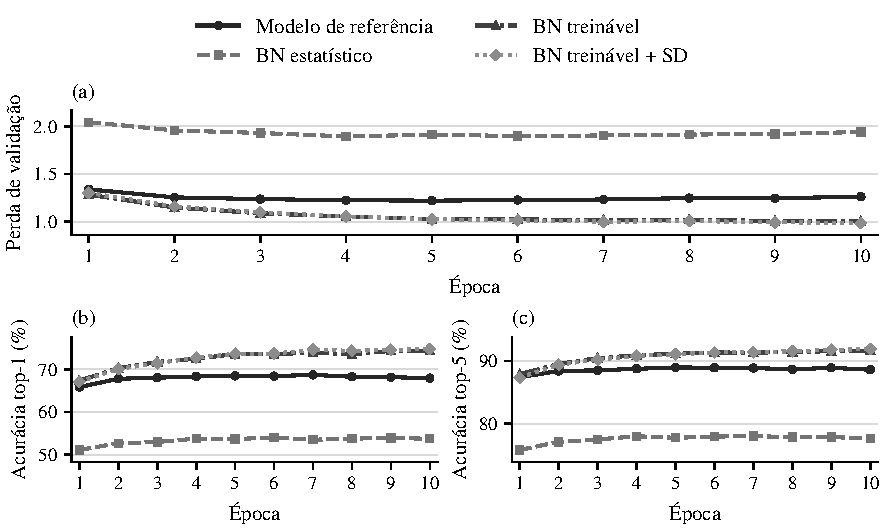
\includegraphics[width=\textwidth]{figures/metricas_validacao.pdf}
  \caption{Métricas de validação por época: (a) perda, (b) acurácia top-1 e
    (c) acurácia top-5. A legenda é compartilhada pelos três painéis.}
  \label{fig:metricas-validacao}
\end{figure}

\section{Discussão}
\label{sec:discussao}

Os resultados mostram que atualizar apenas as estatísticas do Batch
Normalization não melhorou o desempenho neste experimento. Uma hipótese
para a queda observada é que a normalização pelas estatísticas dos lotes
altere as representações do extrator sem permitir a adaptação de seus
parâmetros de escala e deslocamento. O ganho obtido com
BN treinável sugere que ajustar esses parâmetros contribuiu
para adaptar o modelo ao Food-101, mesmo com as convoluções congeladas.
Entretanto, os experimentos realizados não permitem determinar isoladamente
a causa da queda em BN estatístico.

As curvas também mostram diferenças na evolução do aprendizado. No
modelo de referência, a perda de validação atinge seu mínimo na quinta época;
em BN estatístico, na quarta. Em ambos, a perda de validação termina
acima do mínimo observado. Em
BN treinável e BN treinável + SD, a menor perda
de validação ocorre na décima
época, indicando que o treinamento ainda apresentou melhora nesse critério
até o final do período avaliado.

O Stochastic Depth acrescentou um ganho de 0,50 ponto percentual em
acurácia top-1 de teste, sem aumentar a quantidade de parâmetros treináveis.
Sua perda final de validação também foi menor que a de
BN treinável (0,9866 contra 1,0045).

A comparação está limitada a uma execução por configuração, com semente
fixa e duração de 10 épocas. Assim, não é possível estimar a variabilidade
dos resultados entre execuções nem afirmar que o ganho adicional do
Stochastic Depth seja consistente entre sementes. As conclusões se
restringem às configurações e às condições avaliadas.

\section{Conclusões}
\label{sec:conclusoes}

Este trabalho investigou a transferência de aprendizado com EfficientNet-B0
para a classificação de alimentos no Food-101, mantendo os pesos das
convoluções congelados. O treinamento do
classificador em conjunto com os parâmetros de escala e deslocamento do
Batch Normalization, combinado com Stochastic Depth, apresentou o melhor
desempenho: 79,43\% de acurácia top-1 e 94,86\% de acurácia top-5 no
teste. O ganho em top-1 sobre o modelo de referência foi de 6,65 pontos
percentuais. O treinamento dos 42.016 parâmetros adicionais do Batch
Normalization, sem Stochastic Depth, já havia proporcionado um ganho de
6,15 pontos percentuais; a ativação dessa regularização acrescentou
0,50 ponto percentual.

A atualização apenas das médias e variâncias acumuladas apresentou
desempenho inferior ao modelo de referência. Nas condições avaliadas, os
resultados favorecem a adaptação conjunta das estatísticas e dos parâmetros
do Batch Normalization, em vez da atualização exclusiva das estatísticas.
Essa observação se limita ao protocolo adotado, com 10 épocas e uma
semente por configuração, sem permitir estabelecer a estabilidade do ganho
adicional proporcionado pelo Stochastic Depth.

Como continuidade, propõe-se repetir os experimentos com diferentes
sementes, avaliar o treinamento por mais épocas e investigar o
descongelamento parcial das convoluções. Essas comparações poderão
esclarecer a estabilidade dos ganhos observados e o potencial de uma
adaptação mais ampla do modelo ao reconhecimento de alimentos.


\bibliographystyle{sbc}
\bibliography{referencias}

\end{document}
